\documentclass[a4paper]{article}
\usepackage{german}
\usepackage[utf8]{inputenc}

\usepackage{pgfplots}
\usepackage{pgfplots.assert}

\usepgfplotslibrary{fillbetween}

\begin{document}

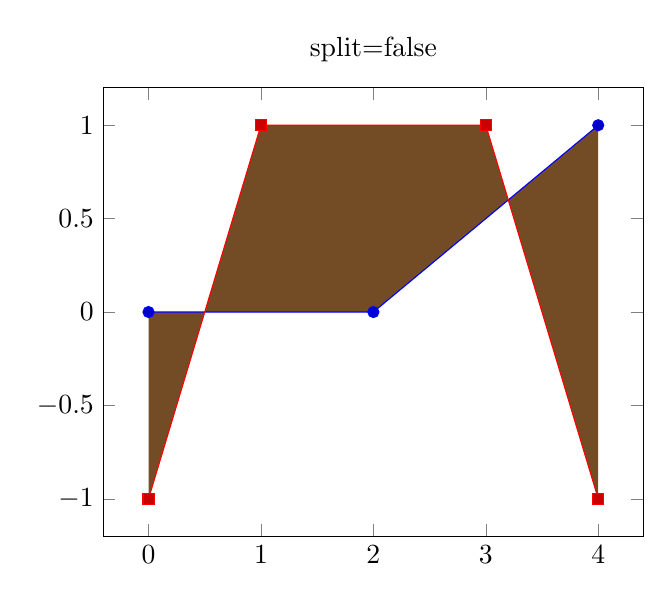
\begin{tikzpicture}
	\begin{axis}[title={split=false}]
	\addplot+[name path=A] coordinates {(0,0) (2,0) (4,1)};
	\addplot+[name path=B] coordinates {(4,-1) (3,1) (1,1) (0,-1)};

	\addplot fill between[of=A and B,
		];

	\end{axis}
\end{tikzpicture}

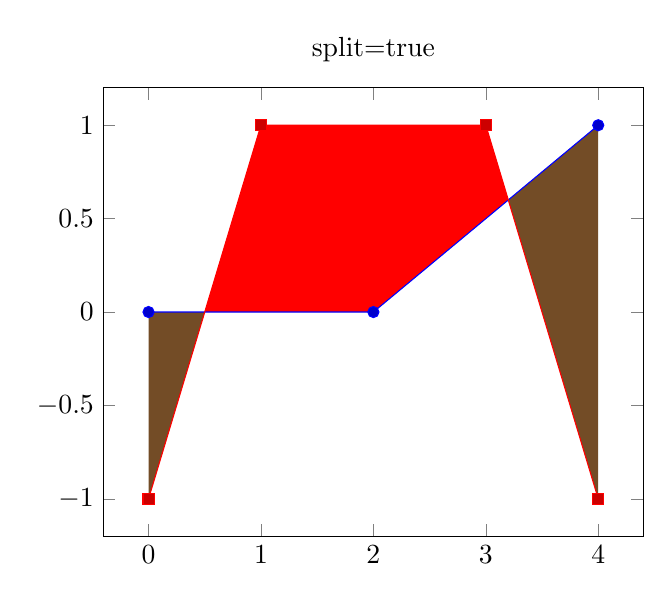
\begin{tikzpicture}
	\begin{axis}[title={split=true}]
	\addplot+[name path=A] coordinates {(0,0) (2,0) (4,1)};
	\addplot+[name path=B] coordinates {(4,-1) (3,1) (1,1) (0,-1)};

	\addplot fill between[of=A and B,
		split,
		every odd segment/.style={fill=red},
		];

	\end{axis}
\end{tikzpicture}

\end{document}

